% ------------------------------------------------------------------------------
% TYPO3 CMS 7.5 - What's New (Russian Version)
%
% @author	Michael Schams <schams.net>
% @license	Creative Commons BY-NC-SA 3.0
% @link		http://typo3.org/download/release-notes/whats-new/
% @language	Russian
% ------------------------------------------------------------------------------
% LTXE-CHAPTER-UID:		c3acb5a9-2f959469-cbb06402-1f9e6566
% LTXE-CHAPTER-NAME:	Backend User Interface
% ------------------------------------------------------------------------------

\section{Backend User Interface}
\begin{frame}[fragile]
	\frametitle{Backend User Interface}

	\begin{center}\huge{Chapter 1:}\end{center}
	\begin{center}\huge{\color{typo3darkgrey}\textbf{Backend User Interface}}\end{center}

\end{frame}

% ------------------------------------------------------------------------------
% LTXE-SLIDE-START
% LTXE-SLIDE-UID:		70ceedd8-1ba03ef8-cb2a48e3-c75bb7cd
% LTXE-SLIDE-ORIGIN:	a6dd927e-ca5773d5-56b681cb-db07be84 English
% LTXE-SLIDE-ORIGIN:	521453c3-22ab1a9f-6ae647f2-33fe0c0c German
% LTXE-SLIDE-TITLE:		Feature: #56282 - Language selector for pageview module
% LTXE-SLIDE-REFERENCE:	Feature-56282-LanguageSelectorForPageviewModule.rst
% ------------------------------------------------------------------------------
\begin{frame}[fragile]
	\frametitle{Backend User Interface}
	\framesubtitle{Language Selector in Module "Pageview"}

	% Note for translators: try to keep the first line in ONE line.
	% If this is not possible, you possibly want to reduce the image height:
	% change width=0.9 to width=0.8 or even smaller (this reduces the height, too).

	\texttt{WEB->View} features a dropdown to select a language for the page preview.\newline
	\smaller
		(can be deactivated by \texttt{mod.SHARED.view.disableLanguageSelector = 1})
	\normalsize

	\begin{figure}
		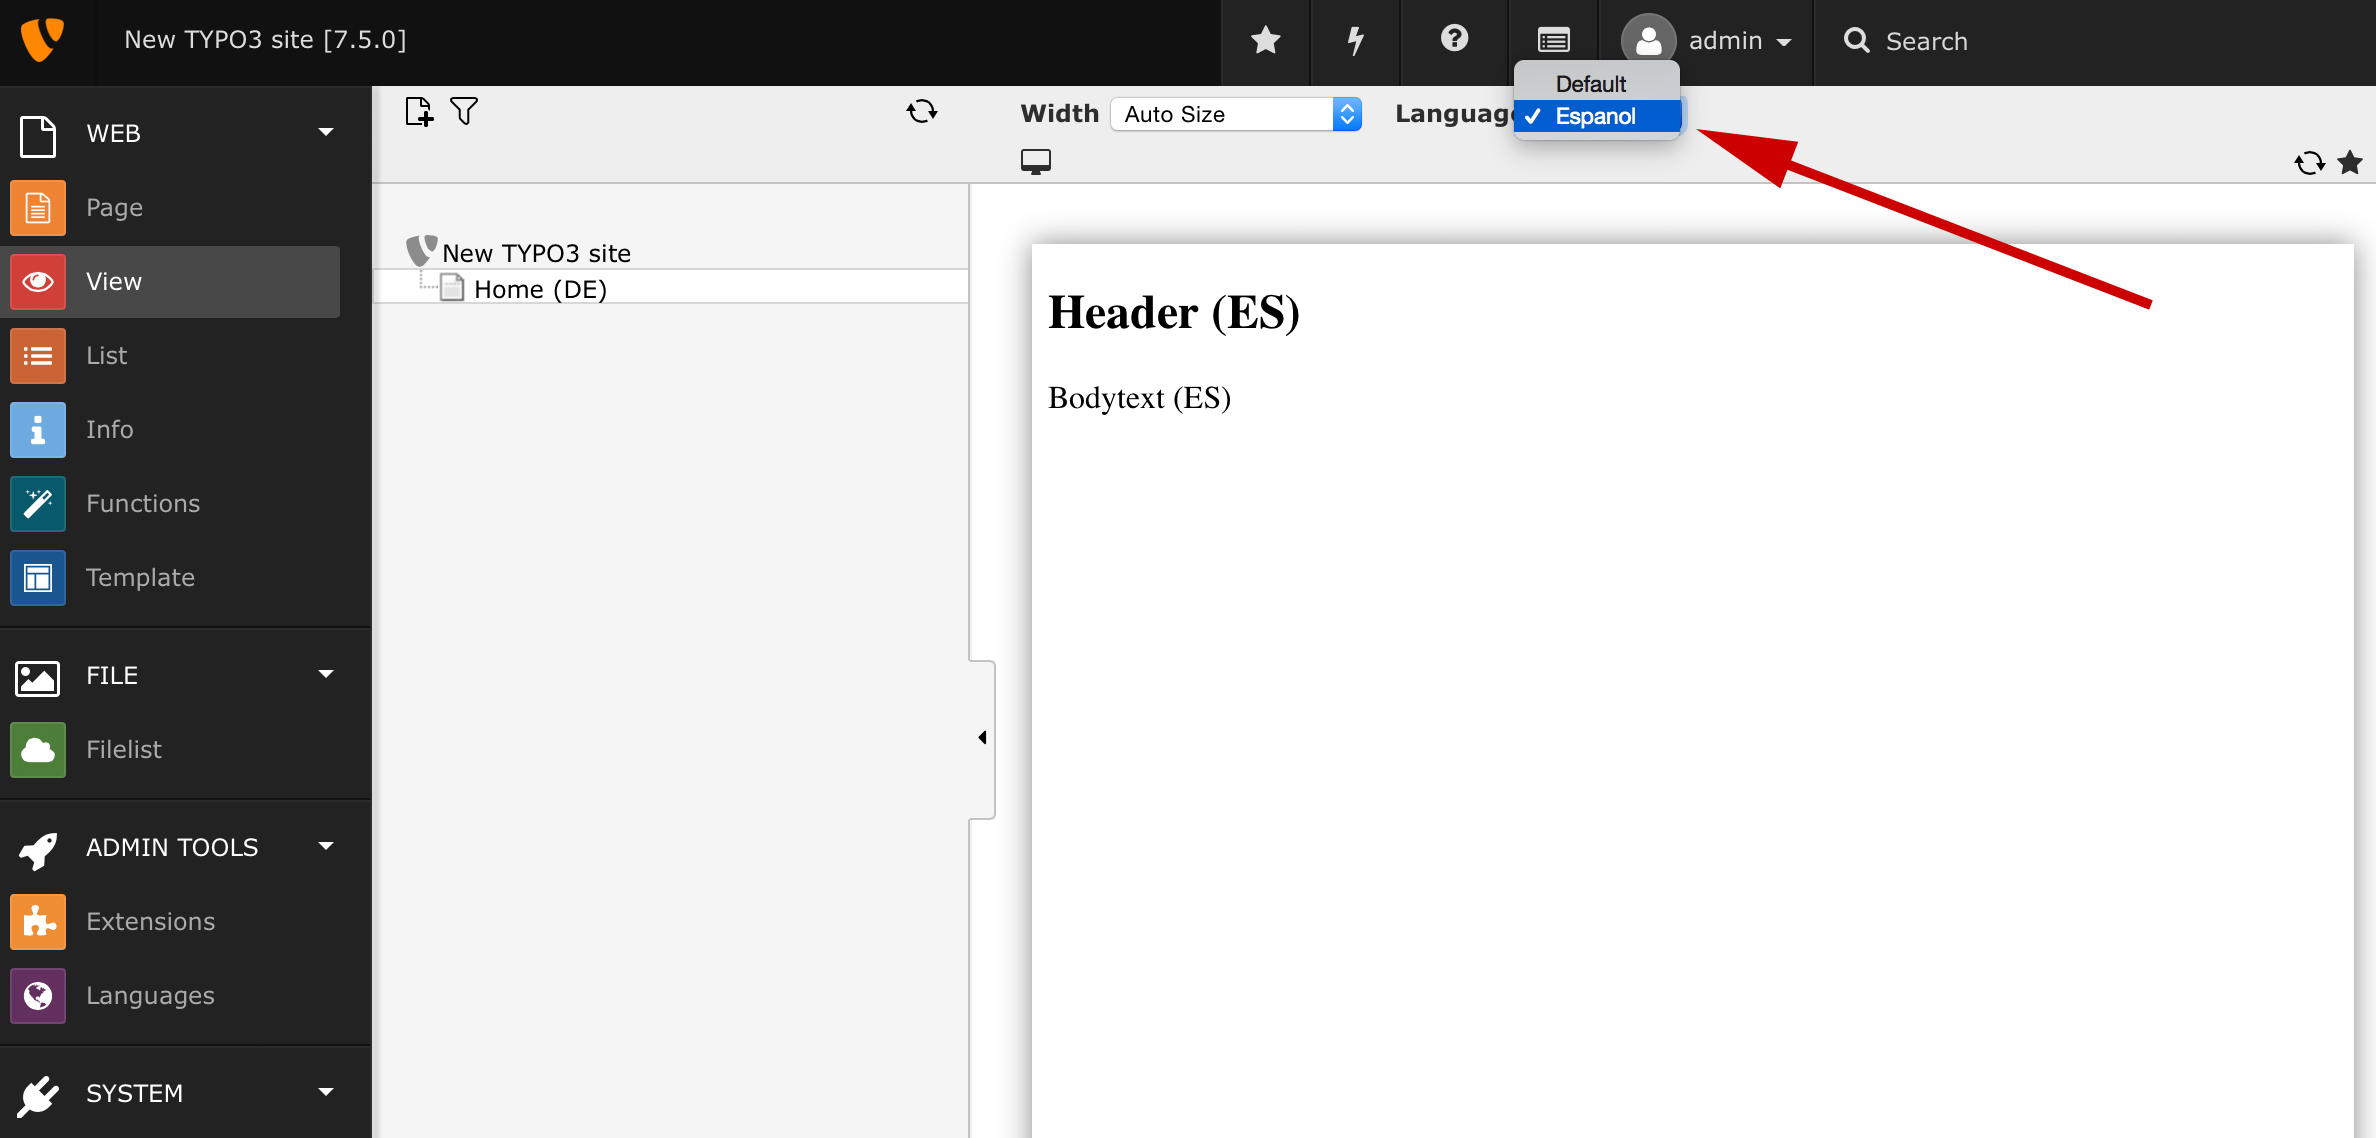
\includegraphics[width=0.9\linewidth]{BackendUserInterface/56282.png}
	\end{figure}

\end{frame}

% ------------------------------------------------------------------------------
% LTXE-SLIDE-START
% LTXE-SLIDE-UID:		efb64bbe-1914b10d-aa8284de-dbcb5889
% LTXE-SLIDE-ORIGIN:	1dc5e5e7-68cbb10e-2477d29f-5d206fc6 English
% LTXE-SLIDE-ORIGIN:	010b80f6-796db221-dbf248bb-89c1e16a German
% LTXE-SLIDE-TITLE:		Feature: #38732 - Fluid-based Content Elements Introduced
% LTXE-SLIDE-REFERENCE:	Feature-38732-Fluid-basedContentElementsIntroduced.rst
% ------------------------------------------------------------------------------
\begin{frame}[fragile]
	\frametitle{Backend User Interface}
	\framesubtitle{Content Element \texttt{textmedia}}

	A new Content Element \textbf{"Text \& Media"} combines the elements
	\texttt{text}, \texttt{image} and \texttt{textpic}.

	\begin{figure}
		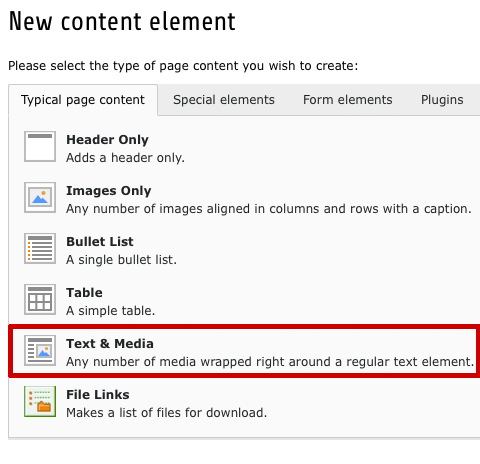
\includegraphics[width=0.5\linewidth]{BackendUserInterface/38732.png}
	\end{figure}

\end{frame}

% ------------------------------------------------------------------------------
% LTXE-SLIDE-START
% LTXE-SLIDE-UID:		13cdfd17-93b4c209-49369069-7c27f333
% LTXE-SLIDE-ORIGIN:	b95bc32c-c073846d-79e2c196-098393c9 English
% LTXE-SLIDE-ORIGIN:	b42c3d82-74137049-3c228477-41e783fb German
% LTXE-SLIDE-TITLE:		Feature: #61799 - Improved handling of online media
% LTXE-SLIDE-REFERENCE:	Feature-61799-ImprovedHandlingOfOnlineMedia.rst
% ------------------------------------------------------------------------------
\begin{frame}[fragile]
	\frametitle{Backend User Interface}
	\framesubtitle{YouTube and Vimeo Files}

	Content Element \textbf{"Text \& Media"} allows editors to include external
	YouTube and Vimeo files, as well as local files.

	\begin{figure}
		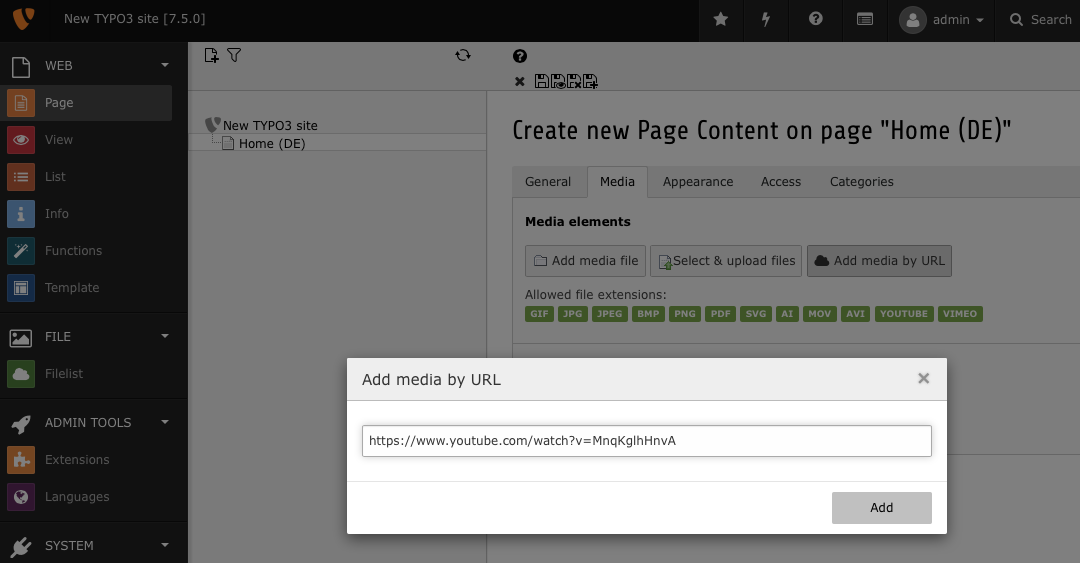
\includegraphics[width=0.75\linewidth]{BackendUserInterface/61799.png}
	\end{figure}

\end{frame}

% ------------------------------------------------------------------------------
% LTXE-SLIDE-START
% LTXE-SLIDE-UID:		3a11ecb7-dd0cb817-8c9a061e-791ffab1
% LTXE-SLIDE-ORIGIN:	3ce8cb92-e6b068e1-8c3d0956-f870bf17 English
% LTXE-SLIDE-ORIGIN:	75cdd96d-aea7b6f1-3b57d603-e990fef9 German
% LTXE-SLIDE-TITLE:		Feature: #69119 - Add a basic search to the filelist module
% LTXE-SLIDE-REFERENCE:	Feature-69119-AddABasicSearchToTheFilelistModule.rst
% ------------------------------------------------------------------------------
\begin{frame}[fragile]
	\frametitle{Backend User Interface}
	\framesubtitle{Search in Module Filelist}

	Module "Filelist" features a search by file name now (recursively from the
	current folder).

	\begin{figure}
		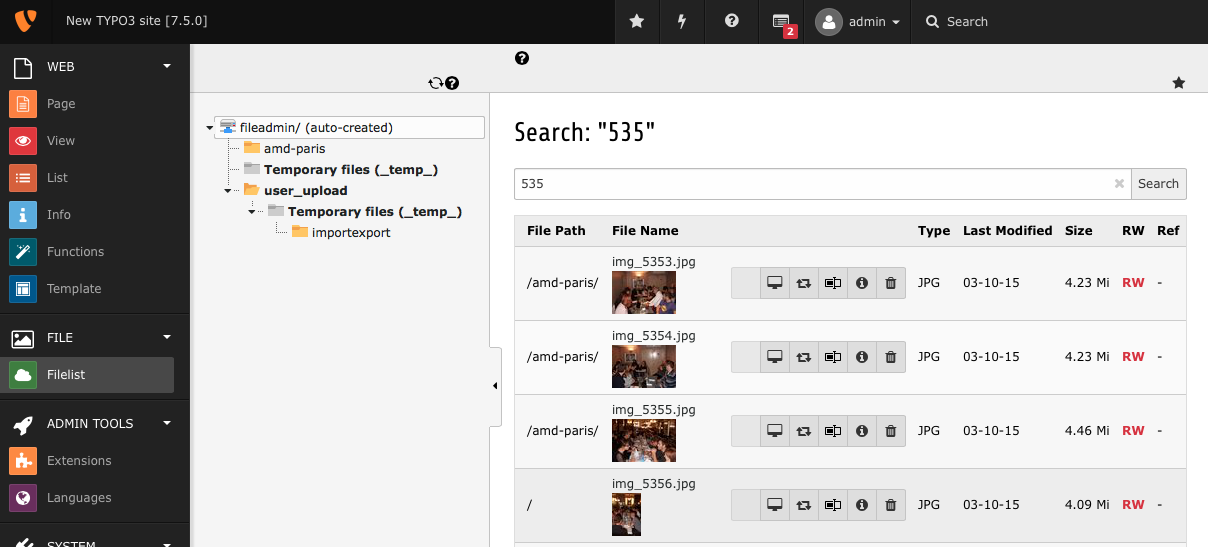
\includegraphics[width=0.9\linewidth]{BackendUserInterface/69119.png}
	\end{figure}

\end{frame}

% ------------------------------------------------------------------------------
